% !TEX root = ../Dokumentation.tex
\subsection{Elektronisches Layout}
Damit über den Mikrocontroller auf die einzelnen elektrischen Komponenten zugegriffen und mit ihnen kommuniziert werden kann, werden diese miteinander verbunden. Dazu werden sie auf eine Leiterplatte geführt welche auf den MCU gesteckt wird.
\\[0.2cm]

\textbf{PCB-Schaltung}\\[0.2cm]
Für die Leiterplatte wurde eine entsprechende Schaltung entworfen, die das Zusammenspiel der elektrischen Hardware ermöglicht. Dabei waren die technischen Spezifikationen der Teile ausschlaggebend für den Entwurf.
So musste beispielsweise gewährleistet werden, dass  keine zu hohen Spannungen auf den Mikrocontroller oder auf andere Komponente geführt werden. Für die Spannungsüberwachung der Akkumulatoren, wurde daher ein Spannungsteiler eingebaut. Mit diesem wird nicht das ganze Potential über den Mikrocontroller geführt, sondern nur ein Wert im vetragbaren Bereich. Bei den Motoren hingegen, wurden DC/DC-Wandler eingesetzt um die Spannung möglichst konstant auf 5V zu halten.
Die Schaltung wurde mithilfe des Altium Designer entworfen und das komplette Schema befindet sich im Anhang.
\\[0.2cm]
\begin{figure}[H]
\centering
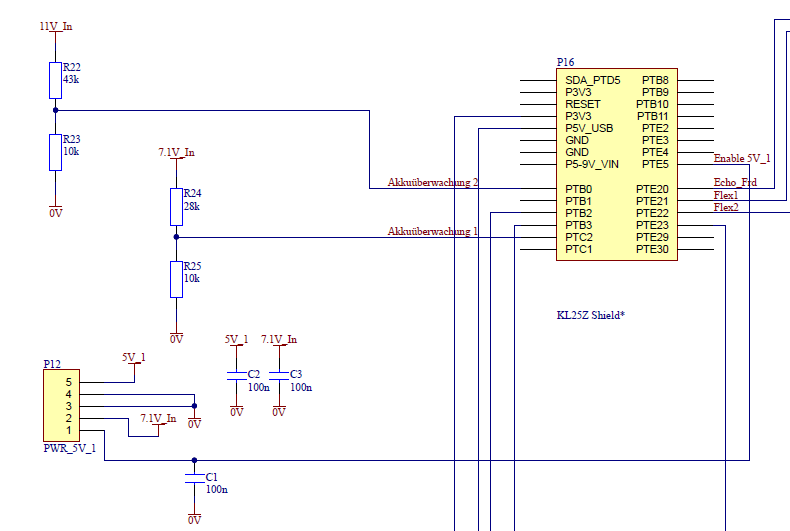
\includegraphics[width=0.5\textwidth]{03_Loesungskonzept/pictures/pcbspannungsteiler.png}
\caption{Spannungsteiler}	
\end{figure}

\textbf{PCB-Layout}
\\[0.2cm]